\section{A Quantitative Metric and Our Key Hypothesis}
\label{sec.metric}
We devised a metric to quantitatively evaluate security aspects of the kernel. 
It addresses a gap in that there is no standard method for properly evaluating 
a system's security level. Thus, enabling fair comparison to be made of different security tools. 
A critical question we investigated, using our metric is: which portions of the kernel are safe and 
contain few bugs? Our framing hypothesis is that \textbf{\textit{commonly used kernel paths}} contain few bugs. 
Our experimental results show that only $2.5\%$ of the historical kernel bugs that we examined were 
found in commonly used kernel paths. Based on this work, we created a new design, so that it 
places only limited trust within the commonly used kernel paths (in \S{4}). Using this new design, we built a prototype 
-- Lind -- as an example of how to use our metric to design and implement secure systems (in \S{5}). 

\begin{table*}[!ht]
\begin{tabular*}{\textwidth}{l @{\extracolsep{\fill}} lc}
\toprule
\multicolumn{3}{c}{Linux Kernel Bugs Examined} \\
\midrule
Vulnerability    &  Specific Type \\
\midrule
 CVE-2014-9529 \cite{CVE:20149529} & concurrency, race condition \\
 CVE-2014-3631 \cite{CVE:20143631} & NULL pointer dereference \\
 CVE-2012-6657 \cite{CVE:20126657} & network socket variable mischeck \\
 CVE-2014-5207 \cite{CVE:20145207} & privilege escalation \\
 CVE-2014-5206 \cite{CVE:20145206} & privilege escalation \\
 CVE-2014-3153 \cite{CVE:20143153} & privilege escalation \\
 CVE-2014-2851 \cite{CVE:20142851} & privilege escalation \\
 CVE-2014-2706 \cite{CVE:20142706} & race condition, DoS \\
 CVE-2014-0100 \cite{CVE:20140100} & race condition, DoS \\
 CVE-2014-0049 \cite{CVE:20140049} & buffer overflow \\
 CVE-2012-6638 \cite{CVE:20126638} & DoS \\
 CVE-2014-0038 \cite{CVE:20140038} & privilege escalation \\
 CVE-2013-6368 \cite{CVE:20136368} & privilege escalation  \\
 CVE-2013-4587 \cite{CVE:20134587} & index error, privilege escalation \\
 CVE-2013-4563 \cite{CVE:20134563} & size/boundary check, DoS \\
 CVE-2013-4348 \cite{CVE:20134348} & value validation error \\
 CVE-2013-4300 \cite{CVE:20134300} & privilege escalation  \\
 CVE-2013-1943 \cite{CVE:20131943} & privilege escalation \\
 CVE-2013-2094 \cite{CVE:20132094} & privilege escalation  \\
 CVE-2013-3301 \cite{CVE:20133301} & NULL pointer dereference, DoS \\
 CVE-2013-1858 \cite{CVE:20131858} & privilege escalation \\
 CVE-2013-1797 \cite{CVE:20131797} & use-after-free \\
 CVE-2013-1763 \cite{CVE:20131763} & privilege escalation, index error \\
 CVE-2013-0310 \cite{CVE:20130310} & NULL pointer dereference \\
 CVE-2012-2136 \cite{CVE:20122136} & heap-based buffer overflow \\
 CVE-2012-2100 \cite{CVE:20122100} & lack of sanity check \\
 CVE-2012-0028 \cite{CVE:20120028} & privilege escalation \\
 CVE-2011-2517 \cite{CVE:20112517} & privilege escalation, buffer overflow \\
 CVE-2012-2123 \cite{CVE:20122123} & privilege escalation \\
 CVE-2012-1146 \cite{CVE:20121146} & NULL pointer dereference \\
 CVE-2012-0207 \cite{CVE:20120207} & divide-by-zero error and panic \\
 CVE-2011-2525 \cite{CVE:20112525} & NULL pointer dereference \\
 CVE-2011-1076 \cite{CVE:20111076} & NULL pointer dereference \\
 CVE-2011-2184 \cite{CVE:20112184} & NULL pointer dereference, none Initialization \\
 CVE-2010-2478 \cite{CVE:20102478} & integer overflow \\
 CVE-2010-2960 \cite{CVE:20102960} & NULL pointer dereference  \\
 CVE-2010-2492 \cite{CVE:20102492} & privilege escalation, buffer overflow \\
 CVE-2010-2240 \cite{CVE:20102240} & stack overflow \\
 CVE-2010-1188 \cite{CVE:20101188} & use-after-free \\
 CVE-2010-0437 \cite{CVE:20100437} & NULL pointer dereference \\
\bottomrule
\end{tabular*}
\caption {Linux Kernel Bugs Examined}
\label{table:kernel_bugs}
\end{table*}

\subsection{Rationale Behind Our Metric}
As discussed previously (in \S{2}), a key reason that existing techniques 
fail to provide strong protection to the kernel is that there has yet to be a good way 
or standard method to understand which portions of the kernel are safe 
and which portions of the kernel are risky. We need to gain more knowledge to answer 
this question to properly decide how should the kernel be exposed to user applications, 
and what could be a good way to protect interactions between the kernel space and 
the user space, without drastic change to the current kernel structure. 
Thus, a metric to help solve this problem is desirable and could have huge practical impact. 

In addition to having a standard method for measuring and evaluating the kernel, 
our metric would also become a solid basis to conduct comparison between different tools that try to 
provide secure environment for running programs. 
Surprisingly, researchers and developers did not have a good way to evaluate the security features 
of their tools, let along conduct comparison between different tools. However, to achieve the 
goal of building and deploying secure systems, it would be very helpful if we could conduct fair and accurate 
comparison between different tools. Our metric provides a quantitative way to 
facilitate such comparison. An example of doing comparison for evaluating security features between different tools is 
demonstrated in our evaluation section (in \S{6}).

\subsection{How Does the Metric Work?}
To evaluate security aspects of the kernel using our metric, there are two key steps. First, 
\textbf{\textit{the kernel trace}} of which lines of code in the kernel get executed needs to be captured. 
Secondly, the kernel trace is checked against the historical kernel bugs to see if it contains kernel vulnerabilities. 

The first step in using our metric is to capture the lines of kernel code get executed. 
The Operating System kernel source code is organized under different kernel paths and folders. 
Whenever system resources, such as I/O, memory, and CPU, need to be accessed, the kernel code 
under corresponding paths will be executed to perform necessary functions. Therefore, the kernel code 
execution can be viewed as the fundamental activities of the kernel, and it reflects the basic behavior of 
the kernel. Thus, it makes sense to measure and analyze which lines of code get executed in the kernel. 
Our metric adopts this fundamental approach. It first captures which lines of code in the kernel get executed 
when running certain task programs, which we called the kernel trace. The kernel trace closely
ties with the set of task programs that generated the trace. Therefore, conducting comparison between 
different tools and environments becomes possible by using the kernel traces. To capture the kernel trace, 
we used a tool called Gcov \yiwen{cite: Gcov}, which is a component inside the Linux kernel.

The next step is to evaluate security aspects of the kernel trace that we captured. Using the historical kernel vulnerability 
reports, we built a list of severe kernel bugs. For each of the bugs we examined, we identified the lines of code 
in the kernel that would trigger the bug. We determine that the lines of code in the kernel are \textit{risky} if they 
may trigger certain kernel vulnerabilities. And those lines of code that cannot trigger kernel vulnerabilities are 
considered to be \textit{safe}. This gives us a precise way to know which portions of the kernel are safe and which 
portions of the kernel are risky. 

\subsection{Key Hypothesis: Commonly Used Kernel Paths Contain Few Bugs}
Now, to address the problem that motivated our metric from the very beginning, which portions of the kernel 
are safe and which portions of the kernel are risky. We can use our metric to answer this question. To be more
specific, we use our metric to get an idea of which lines of code in the kernel contain few bugs, then label 
those lines as safe lines. The safe lines of code would then compose the safe portions of the kernel, which can 
be trusted to build a secure trusted computing base for designs of secure systems (shown in \S{4}). 

Our hypothesis is that commonly used kernel paths are likely to be safe and contain few bugs. 
Here, ``commonly used kernel paths'' refers to the kernel paths executed by running popular and 
daily-used applications, such as Web browser applications, file editor applications, and etc. 
The logic behind our hypothesis is that commonly used kernel paths are used frequently, usually 
on a daily basis, and therefore have been well examined and reinforced by the security community and
the kernel development teams. In addition, commonly used kernel paths usually include 
kernel functions that are used in a normal way rather than special corner cases, which means that the chances 
to harbor kernel bugs in those commonly used kernel paths are slim. 

If our hypothesis can be verified, then it would become a critical guideline to create new designs for secure systems 
(shown in \S{4}). 
But before going too far into the new designs, let us first verify that our hypothesis indeed holds, that 
commonly used kernel paths are likely to contain few bugs and be safe. 

\subsection{Verification of the Key Hypothesis}
Our hypothesis is that commonly used kernel paths contain few bugs. 
So to verify our hypothesis, we first needed to obtain the commonly used kernel paths. 
We generated the commonly used kernel paths by using and combining two approaches, 
system call fuzzing, and running popular user applications. 

User space applications interact with the kernel space essentially through the system call API. 
So all those system calls are at the bottom level, while the applications sit at the top level. 
It makes sense then to obtain the kernel trace from both of those two different levels. 
We used two different approaches to obtain the kernel trace of commonly used kernel paths. 
Experiments of both approaches were conducted using the Native Linux environment.

\textbf{1) the bottom-up approach: system call fuzzing.}
Our system call fuzzing is basically running system calls exhaustively with all possible 
arguments and options. We conducted system call fuzzing over more than 300 available system calls, 
which gave us a thorough kernel trace. 

\textbf{2) the top-down approach: running popular user applications.} 
We ran applications that are commonly used by many users on a daily basis, such as Web browser application
and file editor application.  

\begin{table}[ht]
\centering
\begin{tabular}{|l|c|}
  \hline
  Approach & Kernel Coverage (percentage) \\
  \hline \hline
  System Call Fuzzing & 23\% \\
  \hline
  User Applications & 19\% \\
  \hline
\end{tabular}
\caption {Kernel Coverage}
\label{table:kernel_coverage}
\end{table}

\begin{figure}[h]
\centering
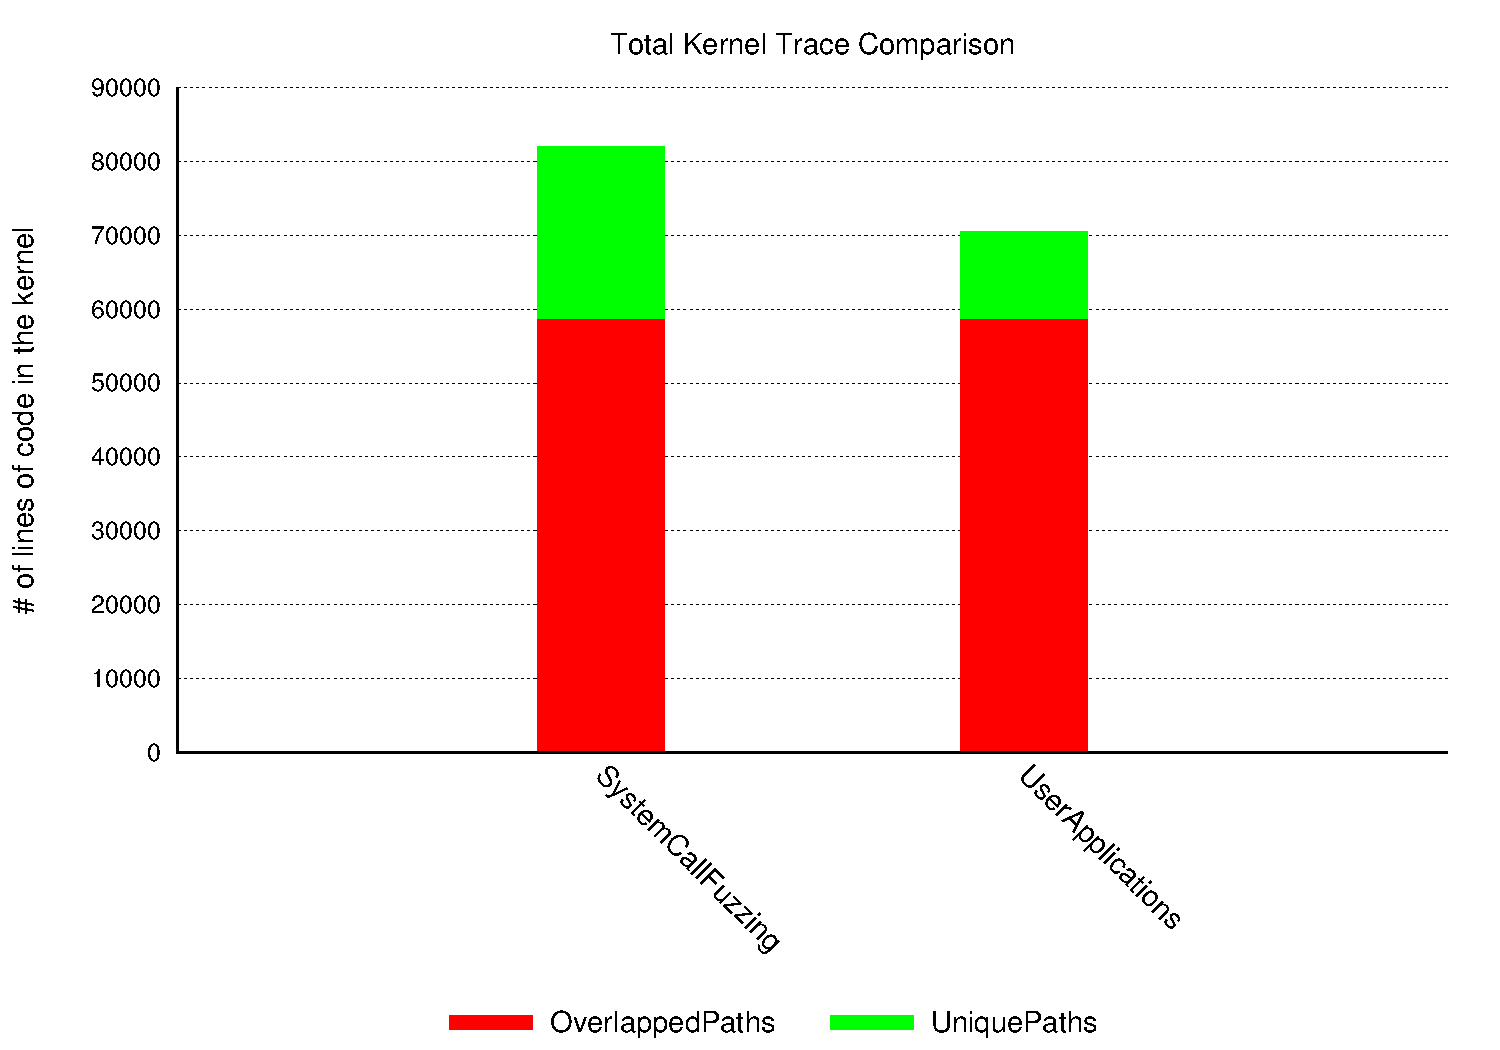
\includegraphics[width=1.0\columnwidth]{diagram/lind_ccs15_diagram_01.pdf}
\caption{Kernel Trace Comparison: Two Approaches}
\label{fig:two_approaches_trace}
\end{figure}

\begin{figure}[h]
\centering
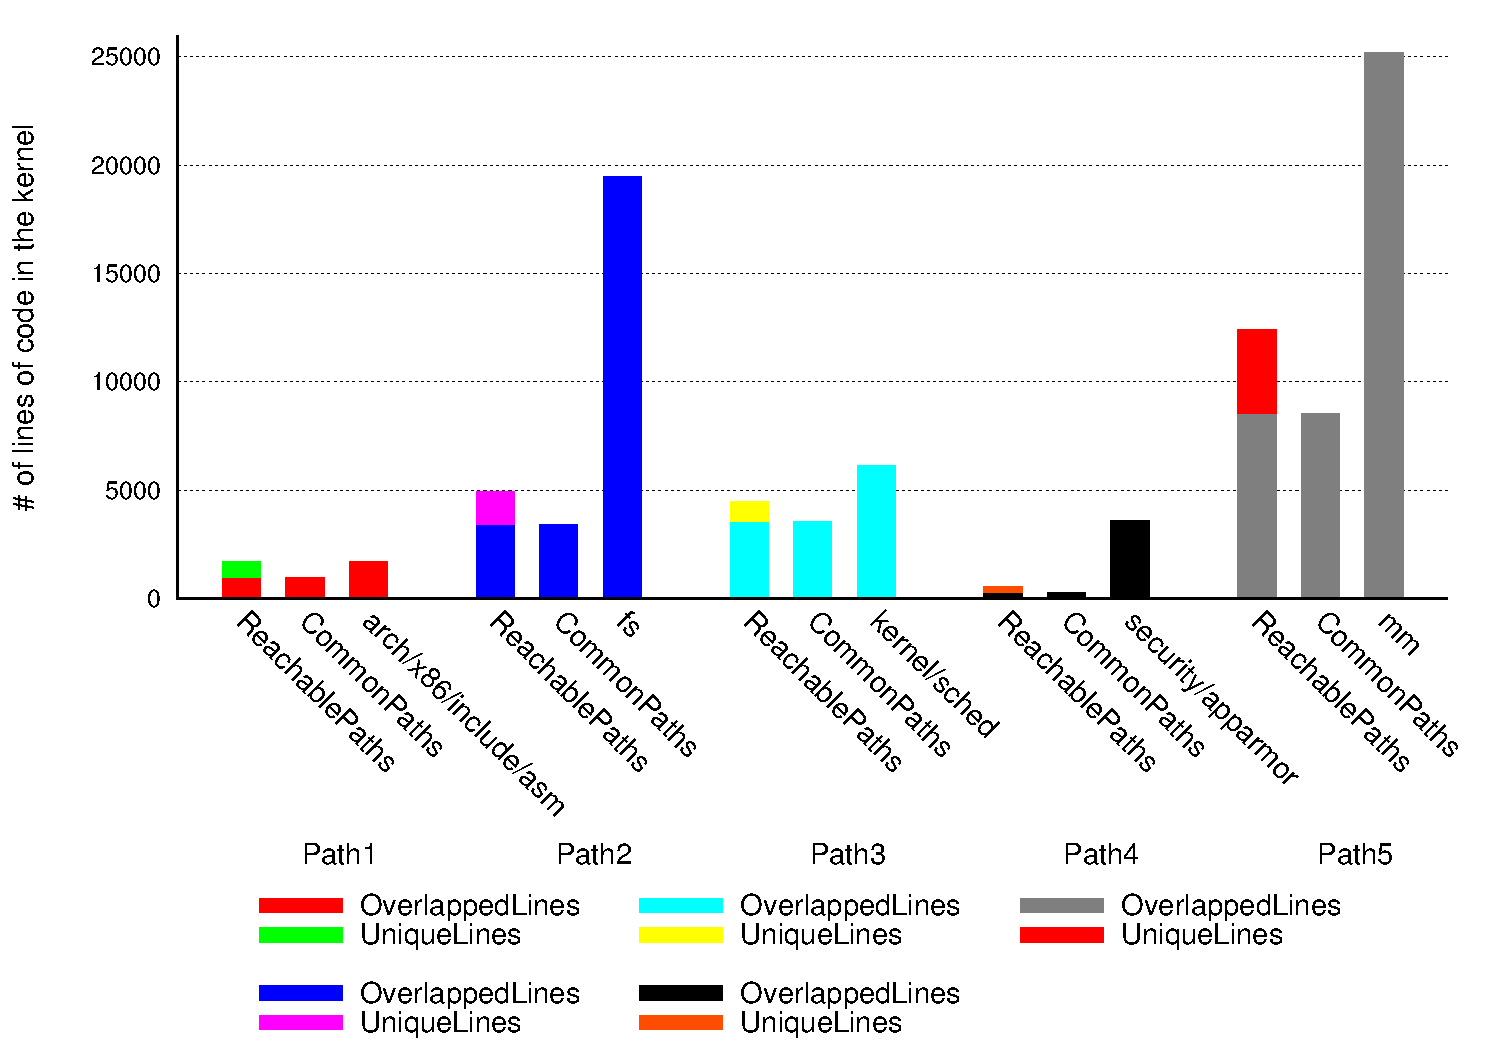
\includegraphics[width=1.0\columnwidth]{diagram/lind_ccs15_diagram_02.pdf}
\caption{Kernel Trace in Key Paths}
\label{fig:key_paths_trace}
\end{figure}

\begin{table*}[!ht]
\begin{tabular*}{\textwidth}{l @{\extracolsep{\fill}} cc}
\toprule
\multicolumn{3}{c}{Vulnerabilities in Commonly Used Kernel Paths} \\
\midrule
& \multicolumn{2}{c}{Commonly Used Kernel Paths} \\
\cline{2-3}
Vulnerability    &  System Call Fuzzing Paths &  User Application Paths \\
\midrule
 CVE-2014-9529 \cite{CVE:20149529} & \ding{55} & \ding{55} \\
 CVE-2014-3631 \cite{CVE:20143631} & \ding{55} & \ding{55} \\
 CVE-2012-6657 \cite{CVE:20126657} & \ding{55} & \ding{55} \\
 CVE-2014-5207 \cite{CVE:20145207} & \ding{55} & \ding{55} \\
 CVE-2014-5206 \cite{CVE:20145206} & \ding{55} & \ding{55} \\
 CVE-2014-3153 \cite{CVE:20143153} & \ding{55} & \ding{55} \\
 CVE-2014-2851 \cite{CVE:20142851} & \ding{55} & \ding{55} \\
 CVE-2014-2706 \cite{CVE:20142706} & \ding{55} & \ding{55} \\
 CVE-2014-0100 \cite{CVE:20140100} & \ding{55} & \ding{55} \\
 CVE-2014-0049 \cite{CVE:20140049} & \ding{55} & \ding{55} \\
 CVE-2012-6638 \cite{CVE:20126638} & \ding{55} & \ding{55} \\
 CVE-2014-0038 \cite{CVE:20140038} & \ding{55} & \ding{55} \\
 CVE-2013-6368 \cite{CVE:20136368} & \ding{55} & \ding{55} \\
 CVE-2013-4587 \cite{CVE:20134587} & \ding{55} & \ding{55} \\
 CVE-2013-4563 \cite{CVE:20134563} & \ding{55} & \ding{55} \\
 CVE-2013-4348 \cite{CVE:20134348} & \ding{55} & \ding{55} \\
 CVE-2013-4300 \cite{CVE:20134300} & \ding{55} & \ding{55} \\
 CVE-2013-1943 \cite{CVE:20131943} & \ding{55} & \ding{55} \\
 CVE-2013-2094 \cite{CVE:20132094} & \ding{55} & \ding{55} \\
 CVE-2013-3301 \cite{CVE:20133301} & \ding{55} & \ding{55} \\
 CVE-2013-1858 \cite{CVE:20131858} & \ding{55} & \ding{55} \\
 CVE-2013-1797 \cite{CVE:20131797} & \ding{55} & \ding{55} \\
 CVE-2013-1763 \cite{CVE:20131763} & \ding{55} & \ding{55} \\
 CVE-2013-0310 \cite{CVE:20130310} & \ding{55} & \ding{55} \\
 CVE-2012-2136 \cite{CVE:20122136} & \ding{55} & \ding{55} \\
 CVE-2012-2100 \cite{CVE:20122100} & \ding{55} & \ding{55} \\
 CVE-2012-0028 \cite{CVE:20120028} & \ding{55} & \ding{55} \\
 CVE-2011-2517 \cite{CVE:20112517} & \ding{55} & \ding{55} \\
 CVE-2012-2123 \cite{CVE:20122123} & \ding{55} & \ding{55} \\
 CVE-2012-1146 \cite{CVE:20121146} & \ding{55} & \ding{55} \\
 CVE-2012-0207 \cite{CVE:20120207} & \ding{55} & \ding{55} \\
 CVE-2011-2525 \cite{CVE:20112525} & \ding{55} & \ding{55} \\
 CVE-2011-1076 \cite{CVE:20111076} & \ding{55} & \ding{55} \\
 CVE-2011-2184 \cite{CVE:20112184} & \ding{55} & \ding{55} \\
 CVE-2010-2478 \cite{CVE:20102478} & \ding{55} & \ding{55} \\
 CVE-2010-2960 \cite{CVE:20102960} & \ding{55} & \ding{55} \\
 CVE-2010-2492 \cite{CVE:20102492} & \ding{55} & \ding{55} \\
 CVE-2010-2240 \cite{CVE:20102240} & {\color{red}\ding{51}} & {\color{red}\ding{51}}\\
 CVE-2010-1188 \cite{CVE:20101188} & \ding{55} & \ding{55} \\
 CVE-2010-0437 \cite{CVE:20100437} & \ding{55} & \ding{55} \\ 
\bottomrule
\end{tabular*}
\caption {Vulnerabilities in Commonly Used Kernel Paths 
({\color{red}\ding{51}}: vulnerability in paths; \ding{55}: vulnerability not in paths)}
\label{table:vulnerabilities_commonly_used_kernel_paths}
\end{table*}

Using the two approaches we just described, we obtained the trace of commonly used kernel paths.
The kernel trace coverage of the two approaches are as shown in Table 2. 
A further breakdown of the composition of the kernel trace is illustrated in Figure 1 and Figure 2.

The results from Table 2 show that the size of commonly used kernel paths is not very large, only about $20\%$ 
of the entire kernel code base. This is a positive sign that shows that commonly used kernel paths are likely to contain 
few bugs, since the coverage of the commonly used kernel paths is small and leaves little space for vulnerabilities to exist. 

The results from Figure 1 and Figure 2 show that for the two different approaches we used, most of the kernel trace was shared 
and under common paths. 
(Shown by the ``OverlappedPaths'' from Figure 1 and ``OverlappedLines'' from Figure 2.) 
This shows that the kernel trace we generated was indeed commonly used, 
so our method to obtain commonly used kernel paths is reasonable. 

We then checked if those commonly used kernel paths contain few kernel bugs.
We examined a list of 40 severe Linux kernel bugs from the last five years (shown in Table 1). 
We used those 40 kernel bugs to check if there are vulnerabilities within the trace of commonly used kernel paths.
The results of our experiment are shown in Table 3.  

From the results, we can see that commonly used kernel paths contain only $2.5\%$ of the bugs we examined 
from the last five years.  
Our results have positive implication that commonly used kernel paths contain few bugs and are safe. 
Our hypothesis and finding provide insights and guidelines for new designs of secure systems. We discuss details of 
a new design in the next section, \S{4}. 